\documentclass[12pt]{report}                  % Times New Roman, 12pt
%\usepackage{gscale_thesis_singlespace} % Single spaced thesis
\usepackage{gscale_thesis_doublespace} % Double spaced thesis
\usepackage{fancyheadings}                   % Header and footer styling
\usepackage{natbib}                               % Bibliography formatting
\usepackage{setspace}                           % Allows double spacing but skips headers/footers
\title{Assurance for Machine Learning systems}
\halftitle{Assurance for Machine Learning systems} % 60 Characters Max. Including Spaces

\author{Milad Hassani}
\shortauthor{M. Hassani} % Used for page header

\dept{computing and software} % The department you are part of; Must be all lower case
\field{computer science} % What field your thesis is in

\prevdegreeone{Ph.D. (Computer Science),\\ McMaster University, Hamilton, Canada}
\prevdegreetwo{Ph.D.} % Just your degree's field

\submitdate{June 2021}
\copyrightyear{2021}

\principaladviser{Dr. Richard Paige} % Your Supervisor
                                % LaTeX variables for preface pages/headers
\setcounter{tocdepth}{1}                        % Limits the TOC to chapter and section names

% Additional packages
\usepackage{graphicx}                                   % Allows the inclusion of figures
\usepackage{subcaption}                               % Allows captions to be added to subfigures
\usepackage[justification=centering]{caption} % Centres caption text
\usepackage[hidelinks]{hyperref}                    % Linking to LaTeX labels and external URLs
\usepackage{array}                                        % Used for table formatting
\newcolumntype{P}[1]{>{\raggedright\let\newline\\\arraybackslash\hspace{0pt}}m{#1}}
\usepackage{booktabs}                                 % Fancy-style tables
\usepackage{longtable}                                 % Allows for tables that are more than one page long
\usepackage{float}                                         % Better figure placement control
\usepackage{enumerate}   
\usepackage[shortlabels]{enumitem}                            % Numbered lists 
\usepackage[shortcuts]{extdash}                  % Allows manual hyphenation of hypenated words
\usepackage{amsmath}                                % Non-standard math symbols
\usepackage{amsfonts}                                % Extended fonts for 
%mathematics
\usepackage{xcolor}
\usepackage{csquotes}                            % Allows quotes
\numberwithin{equation}{section}                 % Numbers equations based on their section

% ********************************
\begin{document}
\beforepreface                                         % Half title page, title page, declaration page   
  \prefacesection{Lay Abstract}

A lay abstract of not more 150 words must be included explaining the key goals and contributions of the thesis in lay terms that is accessible to the general public.                                  % Lay Abstract
  \prefacesection{Abstract}

Machine Learning (ML) has become one of the fastest growing fields of science in recent years. The theories and technologies underpinning ML are used in a vast number of industrial and scientific applications, including banking, security, automotive and healthcare. Although it is becoming more prevalent to use ML technologies in safety critical settings such as healthcare and aerospace, there is still a significant need to assure safety of such systems. In this report, we will first take a look at the foundations of ML and safety. Next we review some of the methods currently developed for safety assurance in ML. We present these methods using a conceptual model based on four stages of ML: Data Management, Model Training, Model Verification and Model Deployment. We identify some of the open research areas associated with each stage.                                       % Abstract
  %%\thispagestyle{empty}
\null\vfill
\begin{center}
%\textbf{Dedications}
%\linebreak
\textsl{Your Dedication \\ Optional second line}
\end{center}
\vfill
                                      % Dedication
  %\prefacesection{Acknowledgements}

Acknowledgements go here.                 % Acknowledgements
  \referencepageswithnotations{notation} % Table of Contents, List of Figures, List of Tables, Notations
  %\referencepages                                 % No notations version (choose one)
\afterpreface                      
  
  
  \chapter{Introduction}

With new developments in Artificial Intelligence (AI) and ML, a growing number of research projects in this field and many companies have started utilizing these methods.
ML methods are also used in many safety critical applications such as Autonomous Vehicles (AVs) and healthcare applications. Therefore, it is very important to have a clear perspective of the safety of such methods in these applications.

In some applications, an erroneous outcome of the ML model has a harmful impact on many lives, for example in medical diagnosis \cite{Foster2014}, loan approval \cite{Lessmann2015}, autonomous vehicles \cite{koopman2016challenges}, and prison sentencing \cite{Berk2015}.
Despite the numerous research papers in this subject, there is still a need to delve deeper and understand the behavior of ML systems in safety critical applications.

One major drawback in using ML algorithms is that they are often treated as a black box and hence, using safety procedures for these methods is sometimes inapplicable \cite{Schwalbe2020}. In a review of automotive software safety methods \cite{Salay2017}, an analysis of ISO-26262 part-6 methods was performed with respect to safety of ML models. This assessment shows that about 40\% of software safety methods do not apply to ML models \cite{Salay2017}.


Safety specifications often assume that behavior of a component is fully specified. Since the training sets used in ML methods are not necessarily complete, they violate this assumption, and some parts of the specification becomes not applicable to the ML components \cite{Salay2017}. 
Most widely used ML frameworks such as Tensorflow \cite{Abadi2016Tensor} \textcolor{red}{are Pytorch and Caffe using a model driven approach??????} and Theano \cite{Al-Rfou} employ a model driven approach in problem solving. Although model driven engineering approach has been successful in safety critical applications such as Automotive industry, the ML models cannot be guaranteed to operate in a safe manner. 

There are two approaches with respect to ML and safety, first is to study safety of ML methods, algorithms, and processes and the second is to use ML methods to improve pre-existing safety assurance procedures.
We will initially follow the first approach and review the literature for the methods applied to standardize and measure the safety of ML methods.

There are inherent performance metrics related to ML methods, such as accuracy and robustness, which can affect their applicability in safety critical applications. ML models can also be dependent to the domain they are trained \cite{Ganin2015}. In addition, other perturbations such as noise, natural and imaging artifacts can cause ML models to function less accurately \cite{Hendrycks2019}.

In this report we will first explore basics of ML in Chapter \ref{chap:ML}. Then in Chapter \ref{chap:safety} we review definition of safety and how assurance cases are structured. Finally in Chapter \ref{chap:literature} we survey the literature on ML assurance and identify some of the open challenges in this area.                  
        \setcounter{figure}{0}
        \setcounter{equation}{0}
        \setcounter{table}{0}
        
%   \chapter{Your Chapter Title}

This is a sample chapter

\section{Referencing}
% These are some sample references to GAMYGDALA~\citep{popescu2014gamygdala} from the ``refernces.bib" file and state effects of cognition~\citep{hudlicka2002time} from the ``reference\_another.bib" file. These references are not in the same .bib file.

\section{Figures}
This is a single image figure (Figure~\ref{fig_singleenv}:

\begin{figure}[ht]
	\centering
	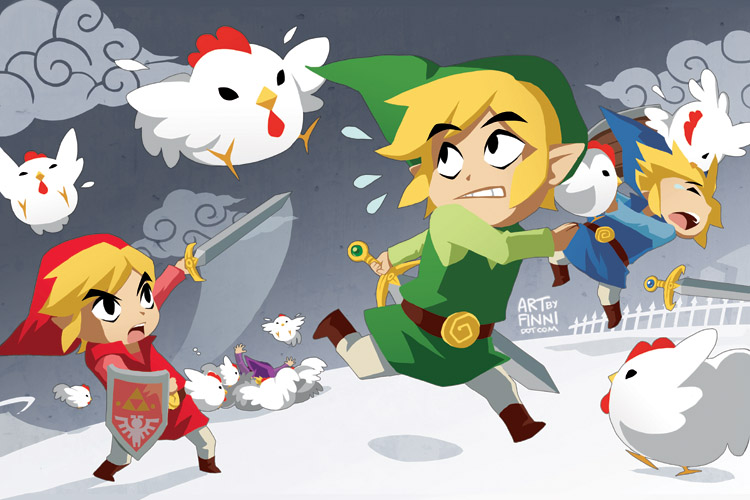
\includegraphics[width=0.6\textwidth]{figures/Sample/tumblr_static_eaceks0rfxsss8o4swscw40wo.jpg}
	\caption[Single Figure Environment Listed Title]{This is a single figure environment}
	\label{fig_singleenv}
\end{figure}

This is a multi-image figure with a top (Figure~\ref{fig_multienv_1}) and bottom (Figure~\ref{fig_multienv_2}) aligned subfigures:

\begin{figure}[ht]
	\centering
	\begin{subfigure}[t]{\textwidth}
		\centering
		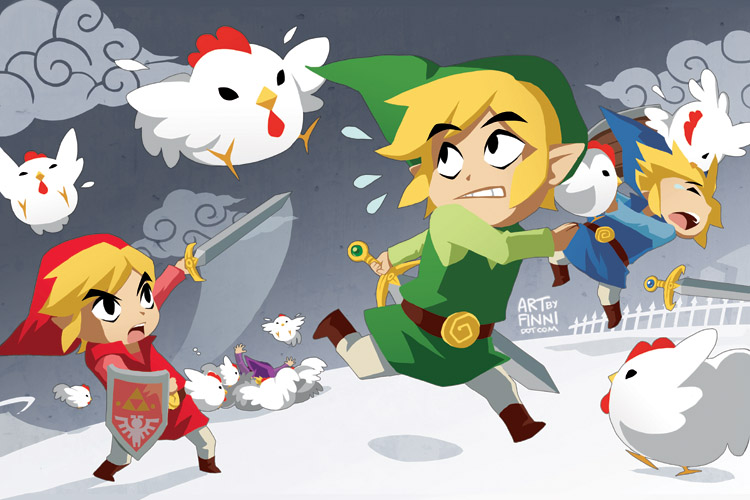
\includegraphics[width=0.7\textwidth]{figures/Sample/tumblr_static_eaceks0rfxsss8o4swscw40wo.jpg}
		\caption{Figure 1}
		\label{fig_multienv_1}
	\end{subfigure}
	~
	\begin{subfigure}[t]{\textwidth}
		\centering
		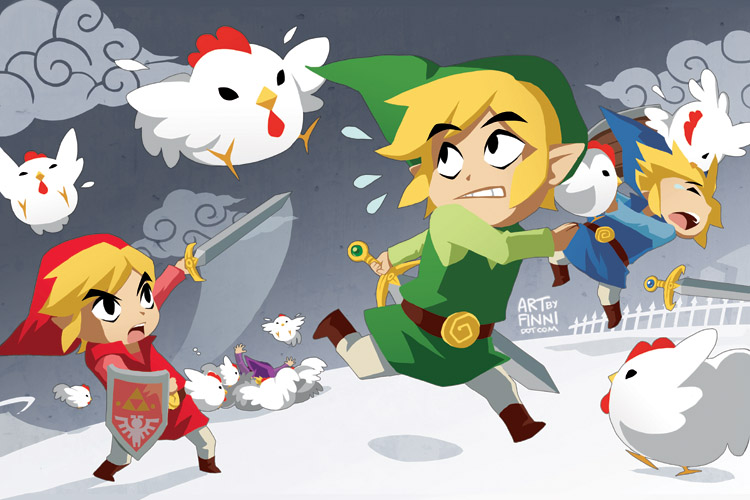
\includegraphics[width=0.7\textwidth]{figures/Sample/tumblr_static_eaceks0rfxsss8o4swscw40wo.jpg}
		\caption{Figure 2}
		\label{fig_multienv_2}
	\end{subfigure}
	
	\caption{A Multi-Figure Environment}
	\label{fig_multienv}
\end{figure}

\section{Tables}

Here is a sample table (Table~\ref{tab_sample}):

	\begin{table}[ht]
	\centering
	\begin{tabular}{ m{0.2\textwidth} m {0.1\textwidth} m{0.15\textwidth} }
		\toprule
		A & $\longleftrightarrow$ & B \\
		C & $\longleftrightarrow$ & D \\
		\bottomrule	
	\end{tabular}	
	\caption{A sample table}	
	\label{tab_sample}
\end{table}

\subsection{Long Tables}
A sample long table is shown in Appendix~\ref{appendix_b}.

\section{Equations}

Here is a sample equation (Equation~\ref{eq_lineslope}):

\begin{equation} \label{eq_lineslope}
	y = mx + b
\end{equation}                  
%        \setcounter{figure}{0}
%        \setcounter{equation}{0}
%        \setcounter{table}{0}

  \chapter{Conclusion}

In this report we first started with the basidc definitions and principals of machine learning and safety assurance concept and eplored some of the fundamentals in both areas in Chapter \ref{chap:ML} and Chapter \ref{chap:safety} we also glanced currently trending research in these areas. Finally, in Chapter \ref{chap:literature} we reviewed some of the literature in assurance of ML systems and some of the open challenges and research questions in this field. 

\textcolor{red}{State some of the major open challenges I found,}
        \setcounter{figure}{0}
        \setcounter{equation}{0}
        \setcounter{table}{0}

% \begin{appendix}
% 	\chapter{Your Appendix}
\label{appendix_a}

Your appendix goes here.

% 		\setcounter{figure}{0}
% 		\setcounter{equation}{0}
% 		\setcounter{table}{0}
		
% 	\chapter{Long Tables}
\label{appendix_b}

This appendix demonstrates the use of a long table that spans multiple pages.

\begin{center}
\begin{longtable}{P{3cm}P{3cm}P{2.5cm}P{3.5cm}}
\toprule
\hline
\textbf{Col A} & \textbf{Col B} & \textbf{Col C} & \textbf{Col D} \\ \midrule

\endfirsthead
\multicolumn{4}{c}{\textit{Continued from previous page}} \\ \hline
\textbf{Col A} & \textbf{Col B} & \textbf{Col C} & \textbf{Col D} \\ \hline
\endhead
\hline \multicolumn{4}{r}{\textit{Continued on the next page}} \\
\endfoot
\hline
\endlastfoot

A & B & C & D \\ \midrule

A & B & C & D \\ \midrule

A & B & C & D \\ \midrule

A & B & C & D \\ \midrule

A & B & C & D \\ \midrule

A & B & C & D \\ \midrule

A & B & C & D \\ \midrule

A & B & C & D \\ \midrule

A & B & C & D \\ \midrule

A & B & C & D \\ \midrule

A & B & C & D \\ \midrule

A & B & C & D \\ \midrule

A & B & C & D \\ \midrule

A & B & C & D \\ \midrule

A & B & C & D \\ \midrule

A & B & C & D \\ \midrule

A & B & C & D \\ \midrule

A & B & C & D \\ \midrule

A & B & C & D \\ \midrule

A & B & C & D \\ \midrule

\hline
\end{longtable}
\end{center}

% 		\setcounter{figure}{0}
% 		\setcounter{equation}{0}
% 		\setcounter{table}{0}
% \end{appendix}

% The bibliography is set up to allow for multiple bib files
\bibliographystyle{plain}
\bibliography{comprehensive,references_another}

\label{NumDocumentPages}

\end{document}
% ********************************
